\graphicspath{{../PR2018/Figures/}}

\title{\fontsize{33}{45}{\huge Pattern Classification (EET 3035)\newline \vspace{8pt} \Large Lecture 06\vspace{-1.1cm}}}
\author{\vspace{-0.4cm}\\\normalsize{\bf Dr. Kundan Kumar}\\ PhD (IIT Kharagpur)\\
Associate Professor\\Department of ECE}
% - Give the names in the same order as the appear in the paper.
% - Use the \inst{?} command only if the authors have different
%   affiliation.

\institute[Indian Institute of Technology Kharagpur] % (optional, but mostly needed)
{

\includegraphics[height=.17\textheight]{SOAlogo.png}\\
 Faculty of Engineering (ITER)\\ S`O'A Deemed to be University, Bhubaneswar, India-751030\\
 \copyright\  2019 Kundan Kumar, All Rights Reserved\\
  \vspace{-1.1cm}}
% - Use the \inst command only if there are several affiliations.
% - Keep it simple, no one is interested in your street address.
\date{}
% To remove page number from a perticular slide
{
\setbeamertemplate{logo}{}
\makeatletter
\setbeamertemplate{footline}{
        \leavevmode%
  
  % First line.
  \hbox{%
  \begin{beamercolorbox}[wd=.2\paperwidth,ht=\beamer@decolines@lineup,dp=0pt]{}%
  \end{beamercolorbox}%
  \begin{beamercolorbox}[wd=.8\paperwidth,ht=\beamer@decolines@lineup,dp=0pt]{lineup}%
  \end{beamercolorbox}%
  } %
  % Second line.
  \hbox{%
  \begin{beamercolorbox}[wd=\paperwidth,ht=\beamer@decolines@linemid,dp=0pt]{linemid}%
  \end{beamercolorbox}%
  } %
  % Third line.
  \hbox{%
  \begin{beamercolorbox}[wd=.1\paperwidth,ht=\beamer@decolines@linebottom,dp=0pt]{}%
  \end{beamercolorbox}%
  \begin{beamercolorbox}[wd=.9\paperwidth,ht=\beamer@decolines@linebottom,dp=0pt]{linebottom}%
  \end{beamercolorbox}%
  }%
        }
\makeatother
\begin{frame}
\titlepage
\end{frame}
}

\section{Linear Discriminant Functions}
\subsection{}
\begin{frame}{}
\begin{variableblock}{\centering \Large \textbf{\vspace{4pt}\newline Linear Discriminant Functions\vspace{4pt}}}{bg=slidecolor,fg=white}{bg=slidecolor,fg=white}
\end{variableblock}
\end{frame}



%\begin{frame}{Introduction}
%\begin{itemize}
%\item In chapter 3, the underlying probability densities were known (or given)
%\item The training sample was used to estimate the parameters of these probability densities (ML, MAP estimations)
%\item In this chapter, we only know the proper forms for the discriminant functions: similar to non-parametric techniques
%\item They may not be optimal, but they are very simple to use
%\item They provide us with linear classifiers
%\end{itemize}
%\end{frame}

\begin{frame}{Linear discriminant functions and decisions surfaces}
\begin{itemize}
\item A discriminant function is a linear combination of the components of ${\rm x}$ can be written as
\begin{equation}
g(x)={\rm w}^T{\rm x}+w_0 \nonumber
\end{equation}
where ${\rm w}$ is the weight vector and $w_0$ the bias or threshold weight.
\item Linear discriminant functions are going to be studied for 
\begin{itemize}
\item the two-category case,
\item multi-category case, and
\item general case
\end{itemize} 
For the general case
there will be $c$ such discriminant functions, one for each of $c$ categories.\nocite{duda2012pattern}
%\item A two-category classifier with a discriminant function of the form (1) uses the following rule:\\
%	Decide $w_1$ if $g(x) > 0$ and $w_2$ if $g(x) < 0$\\
%	Decide $w_1$ if ${\rm w}^tx > -w_0$ and $w_2$ otherwise\\
%	If $g(x) = 0$ then $x$ is assigned to either class
\end{itemize}
\end{frame}

%\begin{frame}{Linear Discriminant Functions}
%\begin{itemize}
%\item A classifier that uses discriminant functions assigns a feature vector ${\rm x}$ to class $\omega_i$ if
%\begin{equation}
%g_i({\rm x})>g_j({\rm x})~~~~\forall j \neq i \nonumber
%\end{equation}
%where $g_i({\rm x})$, $i=1,2,\ldots,c$, are the discriminant functions for $c$ classes.
%\item A discriminant function that is a linear combination of the components of ${\rm x}$ is called a \textit{\color{slidecolor}linear discriminant function} and can be written as
%\begin{equation}
%g({\rm x}) = {\rm w}^T{\rm x}+w_0  \nonumber
%\end{equation}
%where ${\rm w}$ is the \textit{\color{slidecolor}weight vector} and $w_0$ is the \textit{\color{slidecolor}bias} (threshold weight).
%\end{itemize}
%\end{frame}

\section{Two-category}
\subsection{}
\begin{frame}{The Two-Category Case}
\begin{itemize}
\setlength{\itemsep}{12pt}
\item A two-category classifier with a discriminant function of the form $g({\rm x})={\rm w}^T{\rm x}+w_0$ uses the following rule:\\
\begin{equation}
{\sf Decide}~~~~\left\{ {\begin{array}{*{20}{c}}
{{\omega_1}}&{{\sf if}~g({\rm x}) > 0}\\
{{\omega_2}}&{\sf if}~{ g({\rm x}) < 0}
\end{array}} \right.\nonumber
\end{equation}
If $g({\rm x}) = 0$ then ${\rm x}$ is assigned to either class
\item Thus, ${\rm x}$ is assigned to $\omega_1$ if the inner product ${\rm w}^T{\rm x}$ exceeds the
threshold $-w_0$ and to $\omega_2$ otherwise.
\item If $g({\rm x})=0$, ${\rm x}$ can ordinarily be assigned to either class, or can be left undefined.
\end{itemize}
\end{frame}

\begin{frame}{A simple linear classifier}
\begin{figure}
\includegraphics[scale=0.87]{Ch0501}
\caption{A simple linear classifier having $d$ input units, each corresponding to the values of the components of an input vector. Each input feature value $x_i$ is multiplied by its corresponding weight $w_i$; the output unit sums all these products and emits a $+1$ if ${\rm w}^t{\rm x}+w_0>0$ or a $-1$ otherwise}
\end{figure}
\end{frame}

\begin{frame}{The Two-Category Case}
\begin{itemize}
\item The equation $g({\rm x}) = 0$ defines the decision surface that separates points assigned to the category ${\omega_1}$ from points assigned to the category ${\omega}_2$
\item When $g({\rm x})$ is linear, the decision surface is a hyperplane.
%\item Algebraic measure of the distance from ${\rm x}$ to the hyperplane (interesting result!)
\item If ${\rm x}_1$ and ${\rm x}_2$ are both on the decision
surface, then
\begin{align}
{\rm w}^T{\rm x}_1+w_0={\rm w}^T{\rm x}_2+w_0 \nonumber\\
\Rightarrow ~~~~{\rm w}^T({\rm x}_1-{\rm x}_2)=0\nonumber
\end{align}
\item This shows that ${\rm w}$ is normal to any vector lying in the hyperplane.
\end{itemize}
\end{frame}

\begin{frame}{The Two-Category Case}
\begin{itemize}
\item The discriminant function $g({\rm x})$ gives an algebraic measure of the distance from $\rm x$ to the hyperplane. The easiest way to see this is to express ${\rm x}$ as
\begin{equation}
{\rm x} = {{\rm x}_p} + r\frac{{\rm w}}{{\left\| {\rm w} \right\|}} \nonumber
\end{equation}
where ${\rm x}_p$ is the normal projection of ${\rm x}$ onto $H$, and $r$ is the desired algebraic distance which is positive if ${\rm x}$ is on the positive side and negative if ${\rm x}$ is on the negative side.
\item Because, $g({\rm x}_p)=0$
\begin{equation}
r = \frac{{g({\rm x})}}{{\left\| {\rm w} \right\|}} \nonumber
\end{equation}
\end{itemize}
\end{frame}

\begin{frame}{The Two-Category Case}
\begin{itemize}
\item The distance from the origin to $H$ is given by $w_0/\left\| {\rm w} \right\|$. If $w_0>0$, the origin is on the positive side of $H$, and if $w_0<0$, it is on the negative side.
\end{itemize}
\begin{figure}
\includegraphics[scale=0.75]{Ch0502}
\caption{The linear decision boundary $H$, where $g(x)={\rm w}^t{\rm x}+w_0$, separates the feature space into two half-spaces $\mathcal{R}_1$ (where $g({\rm  x})>0$) and $\mathcal{R}_2$ (where $g({\rm x})>0)$)}
\end{figure}
\end{frame}

\begin{frame}{The Two-Category Case}
\begin{itemize}
\item In conclusion, a linear discriminant function divides the feature space by a hyperplane decision surface.
\item The orientation of the surface is determined by the normal vector ${\rm w}$ and the location of the surface is determined by the bias $w_0$.
\item The discriminant function $g({\rm x})$ is proportional to the signed distance from ${\rm x}$ to the hyperplane, with $g({\rm x})>0$ when ${\rm x}$ is on the positive side, and $g({\rm x})<0$ when ${\rm x}$ is on the negative side.
\end{itemize}
\end{frame}

\section{Multi-category}
\subsection{}
\begin{frame}{The multi-category case}
\begin{itemize}
\item There is more than one way to devise multi-category classifiers employing linear discriminant functions.
\begin{columns}
\begin{column}{4cm}
\begin{itemize}
\item c two-class problem
\end{itemize}
\begin{figure}
\includegraphics[scale=0.65]{ldf01}
\end{figure}
\end{column}
\begin{column}{5cm}
\begin{itemize}
\item $c(c-1)/2$ linear discriminants, one for every pair of classes.
\end{itemize}
\begin{figure}
\includegraphics[scale=0.6]{ldf02}
\end{figure}
\end{column}
\end{columns}

\item Pink regions have ambiguous category assignment.
\end{itemize}
\end{frame}

\begin{frame}{The multi-category case}
\begin{itemize}
\item More effective way is to define $c$ linear discriminant functions
\begin{equation}
g_i({\rm x})={\rm w}^t_i{\rm x}+w_0~~~~i=1,2,\ldots,c \nonumber
\end{equation}
	and assign ${\rm x}$ to $\omega_i$ if $g_i({\rm x}) > g_j({\rm x})$ for all $j\neq i$; in case of ties, the classification is undefined
\item In this case, resulting classifier is a ``\textit{\color{slidecolor}linear machine}''.
\item A linear machine divides the feature space into $c$ decision regions, with $g_i({\rm x})$ being the largest discriminant if ${\rm x}$ is in the region $\mathcal{R}_i$
\item For a two contiguous regions $\mathcal{R}_i$ and $\mathcal{R}_j$; the boundary that separates them is a portion of hyperplane $H_{ij}$ defined by:
\begin{equation}
g_i({\rm x})=g_j({\rm x})~~~~~or~~~~~({\rm w}_i-{\rm w}_j)^t{\rm x}+(w_{i0}-w_{j0})=0 \nonumber
\end{equation}
\end{itemize}
\end{frame}

\begin{frame}{The multi-category case}
\begin{itemize}
\item It follows at once that ${\rm w}_i-{\rm w}_j$ is normal to $H_{ij}$, and the signed distance from ${\rm x}$ to $H_{ij}$ is given by 
\begin{equation}
\frac{{({g_i}({\rm x}) - {g_j}({\rm x}))}}{{\left\| {{{\rm w}_i} - {{\rm w}_j}} \right\|}} \nonumber
\end{equation}
\end{itemize}
\begin{figure}
\includegraphics[scale=0.7]{Ch0503}
\caption{Decision boundaries produced by a linear machine for a three-class problem and a five-class problem}
\end{figure}
\end{frame}



%\begin{frame}{The Two-Category Case}
%\begin{itemize}
%\item For the two-category case, the decision rule can be written as
%\begin{equation}
%{\sf Decide}~~~~\left\{ {\begin{array}{*{20}{c}}
%{{\omega_1}}&{{\sf if}~g({\rm x})>0}\\
%{{\omega_2}}&{\sf otherwise~~~~~~~}
%\end{array}} \right.\nonumber
%\end{equation}
%\item The equation $g({\rm x}) = 0$ defines the decision boundary that separates points assigned to $\omega_1$ from points assigned to $\omega_2$.
%\item When $g({\rm x})$ is linear, the decision surface is a hyperplane whose orientation is determined by the normal vector ${\rm w}$ and location is determined by the bias $w_0$.
%\end{itemize}
%\end{frame}

%\begin{frame}{The Multicategory Case}
%\begin{itemize}
%\item There is more than one way to devise multicategory classifiers using linear discriminant functions.
%\item For example, we can reduce the problem as $c$ two-class problems, where the $i$th problem is solved by a linear discriminant that separates points assigned to $\omega_i$ from those not assigned to $\omega_i$.
%\item Alternatively, we can use $c(c-1)/2$ linear discriminants, one for every pair of classes.
%\item Also, we can use $c$ linear discriminants, one for each class, and assign $x$ to $\omega_i$
%if $g_i({\rm x}) > g_j ({\rm x})$ for all $j\neq i$.
%\end{itemize}
%\end{frame}

%\begin{frame}{The Multicategory Case}
%\begin{figure}
%\includegraphics[scale=0.7]{ldf01}~~~~~~~
%\includegraphics[scale=0.7]{ldf02}
%\caption{Linear decision boundaries fro a four-class problem devised as four two-class problems (left figure) and six pairwise problems (right figure). The pink regions have ambiguous category assignments.}
%\end{figure}
%\end{frame}

%\begin{frame}{The Multicategory Case}
%\begin{figure}
%\includegraphics[scale=0.8]{ldf03}
%\caption{Decision boundaries produced by a linear machine for a three-class problem and a five-class problem.}
%\end{figure}
%\end{frame}
\section{Generalized LDF}
\subsection{}
\begin{frame}{Generalized Linear Discriminant Functions}
\begin{itemize}
\item The linear discriminant function $g({\rm x})$ can be written as
\begin{figure}
\includegraphics[scale=1]{ldf04}
\end{figure}
where ${\rm w}=(w_0,w_1,\ldots,w_d)^T$
\item We can obtain the \textit{\color{slidecolor}quadratic discriminant function} by adding second-order terms as
\begin{figure}
\includegraphics[scale=1]{ldf05}
\end{figure}
Because $x_ix_j=x_jx_i$, we can assume that ${\rm w}_{ij}={\rm w}_{ji}$  with no loss in generality. Which result in more complicated decision boundaries.
(hyperquadrics)
\end{itemize}
\end{frame}

\begin{frame}{Generalized Linear Discriminant Functions}
\begin{itemize}
\item The quadratic discriminant function has an additional $d(d+1)/2$ coefficients at its disposal with which to produce more complicated separating surfaces.
\item The separating surface defined by $g({\rm x})=0$ is a second-degree or hyperquadric surface.
\item If the symmetric matrix ${\rm W} = [{\rm w}_{ij}]$, is nonsingular the linear term in $g({\rm x})$ can be eliminated by translating the axes. 
\item The basic character of the separating surface can be described in terms of scaled matrix
\begin{equation}
\bar{\rm W} = \frac{{\rm W}}{{{{\rm w}^t}{{\rm W}^{ - 1}}{\rm w} - 4{w_0}}} \nonumber
\end{equation}
where ${\rm w}=(w_1,\ldots,w_d)^T$ and ${\rm W}=[w_{ij}]$
\end{itemize}
\end{frame}

\begin{frame}{Generalized Linear Discriminant Functions}
The types of quadratic separating surfaces that arise in the general multivariate Gaussian case are as follows
\begin{itemize}
\item[1.] If $\bar{\rm W}$ is a positive multiple of the identity matrix, the separating surface is a \textit{\color{slidecolor}hypersphere} such that $\bar{\rm W}=kI$.
\item[2.] If $\bar{\rm W}$ is positive definite, the separating surfaces is a \textit{\color{slidecolor}hyperellipsoid} whose axes are in the direction of the eigenvectors of $\bar{\rm W}$.
\item[3.] If none of the above cases holds, that is, some of the eigenvalues of are positive and others are negative,
the surface is one of the varieties of types of \textit{\color{slidecolor}hyperhyperboloids}.
\end{itemize}
\end{frame}

\begin{frame}{Generalized Linear Discriminant Functions}
\begin{itemize}
\item By continuing to add terms such as $w_{ijk}x_ix_jx_k$, we can obtain the class of \textit{\color{slidecolor}polynomial discriminant functions}.
These can be thought of as truncated series expansions of some arbitrary $g ( {\rm x} )$, and this in turn suggest the
\textit{\color{slidecolor}generalized linear discriminant function}.
\begin{equation}
g({\rm x}) = \sum\limits_{i = 1}^{\hat d} {{a_i}{{\rm y}_i}(x) = {{\rm a}^t}{\rm y}} \nonumber
\end{equation}
where ${\rm a}$ is a $\hat{d}-$dimensional weight vector and $\hat{d}$ functions ${\rm y}_i({\rm x})$ are arbitrary functions of ${\rm x}$.
\item The physical interpretation is that the functions ${\rm y}_i({\rm x})$ map points ${\rm x}$ in $d$-dimensional space to point ${\rm y}$ in $\hat{d}$-dimensional space.
\end{itemize}
\end{frame}

\begin{frame}{Generalized Linear Discriminant Functions}
\begin{itemize}
\item Then, the discriminant $g({\rm x}) = {\rm a}^t {\rm y}$ separates points in the transformed space using a hyperplane passing through the origin.
\item This mapping to a higher dimensional space brings problems and additional requirements for computation and data.
\item However, certain assumptions can make the problem tractable.
\item Let the quadratic discriminant function be
\begin{equation}
g(x)=a_1+a_2x+a_3x^2 \nonumber
\end{equation}
\item So that the three-dimensional vector ${\rm y}$ is given by
\begin{equation}
{\rm y}=[1~~x~~x^2]^t \nonumber
\end{equation}
\end{itemize}
\end{frame}

\begin{frame}{Generalized Linear Discriminant Functions}
\begin{figure}
\includegraphics[scale=0.8]{ldf06}
\caption{The mapping $y = (1, x, x^2 )^t$ takes a line and transforms it to a parabola
in three dimensions. A plane splits the resulting ${\rm y}$ space into regions corresponding
to two categories, and this in turn gives a non-simply connected decision region in the
one-dimensional $x$ space.}
\end{figure}
\end{frame}

\begin{frame}{Generalized Linear Discriminant Functions}
\begin{figure}
\includegraphics[scale=0.6]{ldf23}
\caption{The two-dimensional input space ${\rm x}$ is mapped through a polynomial
function $f$ to ${\rm y}$. Here the mapping is ${\rm y}_1 = {\rm x}_1$ , ${\rm y}_2 = {\rm x}_2$ and ${\rm y}_3\propto {\rm x}_1 {\rm x}_2$ . A linear
discriminant in this transformed space is a hyperplane, which cuts the surface. Points to the positive side of the hyperplane $\hat{H}$ correspond to category $\omega_1$ , and those beneath
it $\omega_2$ . Here, in terms of the ${\rm x}$ space, $\mathcal{R}_1$ is a not simply connected.}
\end{figure}
\end{frame}

%\begin{frame}{Topics}
%\begin{itemize}
%\item Linear Discriminant Functions and Decision Surfaces
%\item Generalized Linear Discriminant Functions
%\item The two-category linearly separable case
%\item Perceptron Criterion
%\item Criterion Function
%\item Minimum Squared Error Procedures
%\item The Ho-Kashyap Procedures
%\end{itemize}
%\end{frame}
%
%
%\begin{frame}{Introduction}
%\begin{itemize}
%\item Linear Discriminant Functions and Decisions   Surfaces
%\item Generalized Linear Discriminant Functions
%\end{itemize}
%\end{frame}
%

\section{Support Vector Machine}
\subsection{}
\begin{frame}{}
\begin{variableblock}{\centering \Large \textbf{\vspace{4pt}\newline Support Vector Machine\vspace{4pt}}}{bg=slidecolor,fg=white}{bg=slidecolor,fg=white}
\end{variableblock}
\end{frame}

\begin{frame}{Finding ${\rm w}$ with large margin}
\begin{itemize}
\item Let ${\rm x}_n$ be the nearest data point to the plane ${\rm w}^T{\rm x}=0$. \item How far is it?
\item Preliminary technicalities
\begin{itemize}
\item Normalize ${\rm w}$:
\[|{\rm w}^T{\rm x}_n|=1\]
\item Pull out $w_0$:
\[{\rm w}=(w_1,\ldots,w_d) ~~~~~~~ \text{apart from}~~ b\]
The plane is now~~ $\boxed{{\rm w}^T{\rm x}+b=0}$ ~~~(no $x_0$)
\end{itemize}
\end{itemize}
\end{frame}

\begin{frame}{Computing the distance}
\begin{columns}
\begin{column}{6cm}
\begin{itemize}
\item The distance between ${\rm x}_n$ and the plane ${\rm w}^T{\rm x}+b=0$, where $|{\rm w}^{T}{\rm x}_n+b|=1$.
\item The vector ${\rm w}$ is $\perp$ to the plane in the $\mathcal{X}$ space:
\item Take ${\rm x}'$ and ${\rm x}''$ on the plane
\[{\rm w}^T{\rm x}'+b=0~~\text{and}~~{\rm w}^T{\rm x}''+b=0\]
\[\Rightarrow~~ {\rm w}^T({\rm x}'-{\rm x}'')=0\]
\end{itemize}
\end{column}
\begin{column}{5cm}
\begin{figure}
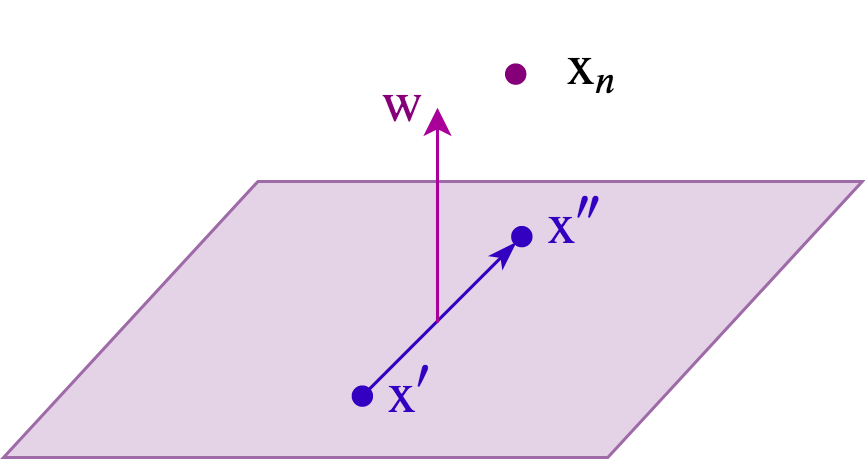
\includegraphics[scale=0.15]{Figures/SVM01.png}
\end{figure}
\end{column}
\end{columns}
\end{frame}

\begin{frame}{Computing the distance}
The distance between ${\rm x}_n$ and the plane:
\begin{columns}
\begin{column}{4cm}
\begin{figure}
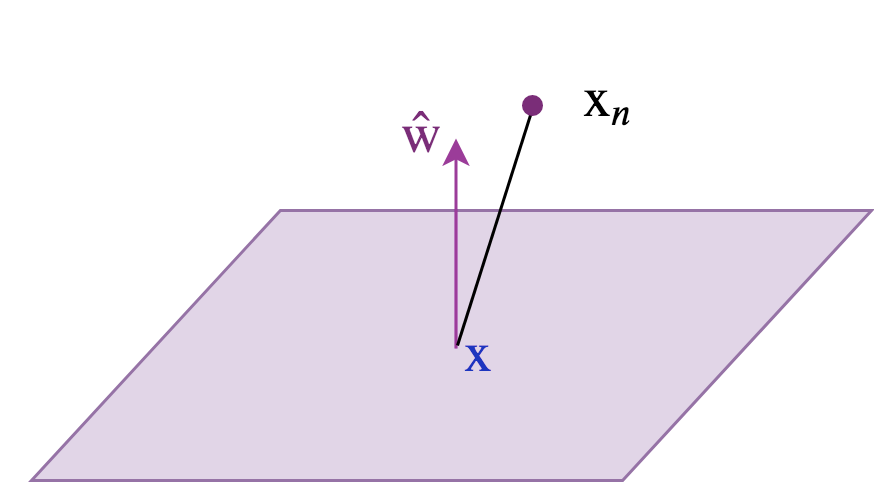
\includegraphics[scale=0.6]{Figures/SVM02.png}
\end{figure}
\end{column}
\begin{column}{6cm}
\begin{itemize}
\item Take any point ${\rm x}$ on the plane
\item Projection of ${\rm x}_n-{\rm x}$ on ${\rm w}$
\[\hat{\rm w}=\frac{\rm w}{||\rm w||}\]
\[\Rightarrow ~~\text{distance}=|\hat{\rm w}^T({\rm x}_n-{\rm x})|\]
%
%${\rm w}^T{\rm x}+b=0$, where $|{\rm w}^{T}{\rm x}_n+b|=1$.
%\item The vector ${\rm w}$ is $\perp$ to the plane in the $\mathcal{X}$ space:
%\item Take ${\rm x}'$ and ${\rm x}''$ on the plane
%\[{\rm w}^T{\rm x}'+b=0~~\text{and}~~{\rm w}^T{\rm x}''+b=0\]
%\[\Rightarrow~~ {\rm w}^T({\rm x}'-{\rm x}'')=0\]
\end{itemize}

\end{column}
\end{columns}
\[\text{distance} = \frac{1}{||{\rm w}||}|{\rm w}^T{\rm x}_n-{\rm w}^T{\rm x}|= \frac{1}{||{\rm w}||}|{\rm w}^T{\rm x}_n+b-{\rm w}^T{\rm x}-b|=\frac{1}{||{\rm w}||}\]
\end{frame}

\begin{frame}{The optimization problem}
\begin{align*}
&\text{Maximize}~~\frac{1}{{\left\| {\rm w} \right\|}}\\
&\text{subject to}\mathop {\min }\limits_{n = 1,2, \ldots N} \left| {{{\rm w}^T}{{\rm x}_n} + b} \right| = 1~~~~~~~~~~~~~~~~~~~~~~~~
\end{align*}
Notice: $\left| {{{\rm w}^T}{{\rm x}_n} + b} \right|=y_n( {{{\rm w}^T}{{\rm x}_n} + b} )$

\begin{align*}
&\text{Minimize}~~\frac{1}{2}{\rm w} ^T{\rm w}\\
&\text{subject to}~~y_n( {{{\rm w}^T}{{\rm x}_n} + b} ) \geq 1~~~~for~~~n=1,2,\ldots,N
\end{align*}
\end{frame}



\begin{frame}{Constrained optimization}
\begin{figure}
\includegraphics[width=\textwidth]{SVM03}
\end{figure}
\end{frame}

\begin{frame}{We saw this before}
\begin{figure}
\includegraphics[width=\textwidth]{SVM04}
\end{figure}
\end{frame}

\begin{frame}{Lagrange formulation}
\begin{figure}
\includegraphics[width=\textwidth]{SVM05}
\end{figure}
\end{frame}

\begin{frame}{Substituting...}
\begin{figure}
\includegraphics[width=\textwidth]{SVM06}
\end{figure}
\end{frame}


\begin{frame}{The solution - quadratic programming}
\begin{figure}
\includegraphics[width=\textwidth]{SVM07}
\end{figure}
\end{frame}


\begin{frame}{QP hand us $\alpha$}
\begin{figure}
\includegraphics[width=\textwidth]{SVM08}
\end{figure}
\end{frame}


\begin{frame}{Support vectors}
\begin{figure}
\includegraphics[width=\textwidth]{SVM09}
\end{figure}
\end{frame}

\begin{frame}{${\rm z}$ instead of ${\rm x}$}
\begin{figure}
\includegraphics[width=\textwidth]{SVM20}
\end{figure}
\end{frame}

\begin{frame}{"Support vectors" in $\mathcal{X}$ space}
\begin{figure}
\includegraphics[width=\textwidth]{SVM21}
\end{figure}
\end{frame}

\begin{frame}{Kernel Trick: What do we need from the $\mathcal{Z}$ space?}
\begin{figure}
\includegraphics[width=\textwidth]{SVM10}
\end{figure}
\end{frame}

\begin{frame}{Generalized inner product}
\begin{figure}
\includegraphics[width=\textwidth]{SVM11}
\end{figure}
\end{frame}

\begin{frame}{The trick}
\begin{figure}
\includegraphics[width=\textwidth]{SVM12}
\end{figure}
\end{frame}

\begin{frame}{The polynomial kernel}
\begin{figure}
\includegraphics[width=\textwidth]{SVM13}
\end{figure}
\end{frame}

\begin{frame}{We only need $\mathcal{Z}$ to exist!}
\begin{figure}
\includegraphics[width=\textwidth]{SVM14}
\end{figure}
\end{frame}

\begin{frame}{This kernel in action}
\begin{figure}
\includegraphics[width=\textwidth]{SVM15}
\end{figure}
\end{frame}

\begin{frame}{Kernel formulation of SVM}
\begin{figure}
\includegraphics[width=\textwidth]{SVM16}
\end{figure}
\end{frame}

\begin{frame}{The final hypothesis}
\begin{figure}
\includegraphics[width=\textwidth]{SVM17}
\end{figure}
\end{frame}

\begin{frame}{How do we know that $\mathcal{Z}$ exists...}
\begin{figure}
\includegraphics[width=\textwidth]{SVM18}
\end{figure}
\end{frame}

\begin{frame}{Design your own kernel}
\begin{figure}
\includegraphics[width=\textwidth]{SVM19}
\end{figure}
\end{frame}

\begin{frame}{Two types of non-separable}
\begin{figure}
\includegraphics[width=\textwidth]{SVM22}
\end{figure}
\end{frame}

\begin{frame}{Error measure}
\begin{figure}
\includegraphics[width=\textwidth]{SVM23}
\end{figure}
\end{frame}

\begin{frame}{The new optimization}
\begin{figure}
\includegraphics[width=\textwidth]{SVM24}
\end{figure}
\end{frame}

\begin{frame}{Lagrange formulation}
\begin{figure}
\includegraphics[width=\textwidth]{SVM25}
\end{figure}
\end{frame}

\begin{frame}{and the solution is ...}
\begin{figure}
\includegraphics[width=\textwidth]{SVM26}
\end{figure}
\end{frame}

\begin{frame}{Types of support vectors}
\begin{figure}
\includegraphics[width=\textwidth]{SVM27}
\end{figure}
\end{frame}

\begin{frame}{Two technical observations}
\begin{figure}
\includegraphics[width=\textwidth]{SVM28}
\end{figure}
\end{frame}

\section{References}
\subsection{}
\begin{frame}[allowframebreaks]{References}
\linespread{1}
\footnotesize
\printbibliography[heading=none]
\end{frame}
{
\nocite{Daugman1985}\nocite{Petkov1995}\nocite{Petkov1997}\nocite{Kruizinga1999}\nocite{Grigorescu2002}\nocite{Petkov2003}\nocite{Grigorescu2003}\nocite{Jain1991}
\setbeamertemplate{logo}{}
\makeatletter
\setbeamertemplate{footline}{
        \leavevmode%
  
  % First line.
  \hbox{%
  \begin{beamercolorbox}[wd=.2\paperwidth,ht=\beamer@decolines@lineup,dp=0pt]{}%
  \end{beamercolorbox}%
  \begin{beamercolorbox}[wd=.8\paperwidth,ht=\beamer@decolines@lineup,dp=0pt]{lineup}%
  \end{beamercolorbox}%
  } %
  % Second line.
  \hbox{%
  \begin{beamercolorbox}[wd=\paperwidth,ht=\beamer@decolines@linemid,dp=0pt]{linemid}%
  \end{beamercolorbox}%
  } %
  % Third line.
  \hbox{%
  \begin{beamercolorbox}[wd=.1\paperwidth,ht=\beamer@decolines@linebottom,dp=0pt]{}%
  \end{beamercolorbox}%
  \begin{beamercolorbox}[wd=.9\paperwidth,ht=\beamer@decolines@linebottom,dp=0pt]{linebottom}%
  \end{beamercolorbox}%
  }%
        }
\makeatother

\begin{frame}
\centering

\includegraphics[width=0.4\paperwidth]{queries.jpg}\\

\includegraphics[width=0.5\paperwidth]{thank_you.png}
\end{frame}
}

